\subsection{Server-side}
\label{sec:remote services}

The remote services of VRDAVis are composed of all the systems that serve the front-end applications; consisting of a data server and a signalling server. 
The data server receives requests from the user application, where its purpose is to transfer data from astronomy data files. 
The signalling server is used to create and manage peer-to-peer connections between two instances of the front-end browser application. 
The peer-to-peer connection is used to transfer the state of the visualisation across instances, allowing the user to transfer the state from a desktop computer to a standalone VR device and vice versa. 
This showcases how VRDAVis would be able to integrate into an astronomer's workflow with minimal disturbance.
% The main purpose of the server-side systems is to serve requests from the front-end clients. 

\subsubsection{Data Server}
% preprocessed files
% cite the CARTA HDF5 papers
% point out that there is a converter from FITS to HDF5
It is common in astronomy for data to be stored in the FITS format.
But in VRDAVis the HDF5 file format will be used to store data. 
Unlike FITS files, where data must be read sequentially, the HDF5 format allows any part of the file to be accessed at any point in time. %cite
The HDF5 C++ library is used to read the files. 
Initially written in C, the C++ package encapsulates the Python code into a format that can be interfaced with C++.

However, merely using a more effective file type is not provide speed-up for creating a visualisation of the stored data. 
Especially when the data in the file is still at its original resolution and therefore its largest size. 
It has the potential to overwhelm the client device with the sheer amount of data it would need to process.
The full-resolution data must be processed into multiple levels of resolution, referred to as mipmaps. 
These mipmaps are contained in the same HDF5 file as the data at its original resolution. 
Portions of the mipmaped data are read, instead reading the full-resolution data, decreasing the likelihood of overwhelming a client device.
% mention that the FITS to HDF5 converter also does the mipmap conversions
% cite the git repo

The server stores the data files pre-processed into a mipmaped format.
This approach to handling \textit{Big Data} files allows the entire dataset to be visualised with less computational overhead, compared to rendering the full resolution dataset~\cite{Li2016}. 
It still allows the visualisation to maintain the overall context of the data, but as the data is explored, higher resolution versions of the same region can be swapped out to allow the user to observe the details.

% insert diagram of how the preprocessed cubelets are stored in the server
\begin{figure*}
    \centering
    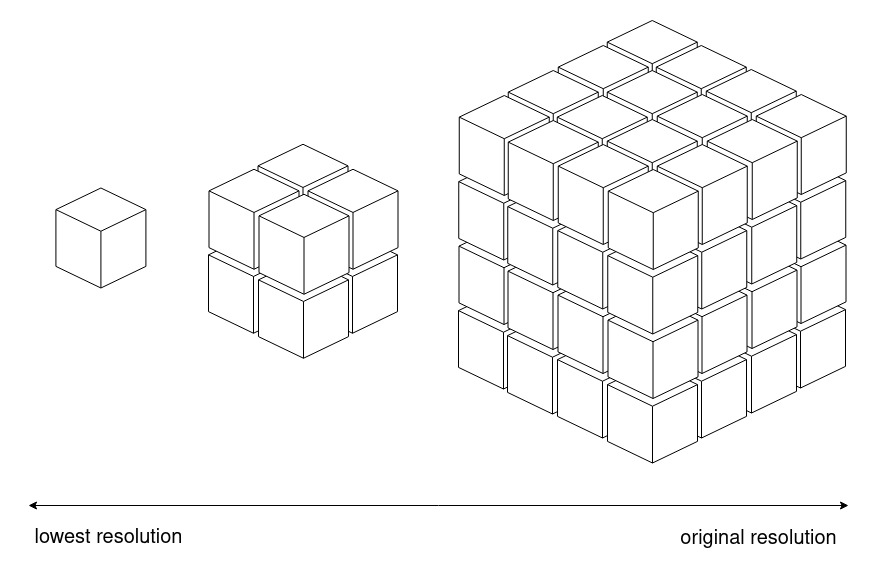
\includegraphics[width=0.6\linewidth]{figures/three-dimensional-mipmap.jpg}
    \caption{In the pre-processed data file, different resolutions are stored as mipmaps, from a single cubelet which represents the entire data cube to the original full-resolution data, with several intermediate levels.}
    \label{fig:three-dimensional-mipmap}
\end{figure*}

\begin{figure*}
    \centering
    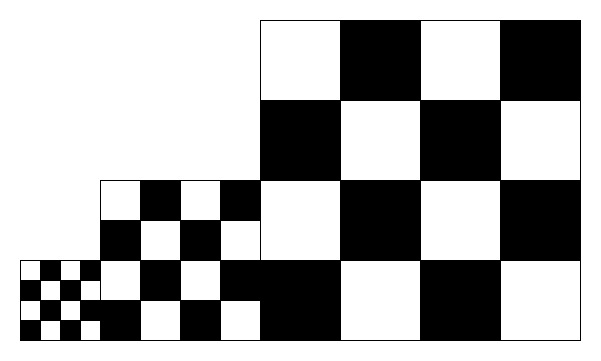
\includegraphics[width=0.5\linewidth]{figures/two-dimensional-mipmap.jpg}
    \caption{An example of a two-dimensional mipmap. Observe how the pattern is scaled at each level}
    \label{fig:two-dimensional-mipmap}
\end{figure*}

% mipmap
% \cite{Li2016}
% The displays on which the visualisations are rendered have a limited number of pixels, thus the lowest granularity possible is to plot one data point onto one pixel (Molina-Solana et al.2017; Olshannikova et al.2015; Yang et al.2015). 
% Visualisation tools are required to “squeeze a billion records into a million pixels”(Bikakis2018) empha-sizing the need for summarisation of data, particularly when creating visualisations

The server must fetch data from its filesystem according to the client's request. 
When the client requests a number of sub-sections of a data cube, the server retrieves these cubes or cubelets and streams them back to the client over a websocket connection. 
Each message streamed to the client contains one compressed cubelet. 
Additionally, the server performs file system functions such as sending lists of available files, opening them, and reading data.

The ability to view various analytics on the visualised data is also an important feature, and the server supports this by computing various derived values such as minimum, maximum, and median values. 
It also compiles analytics data to be visualised as various graphs, including the distribution of values.
%   fetches data based on the client's request
%       client requests a number of cubes but the server streams back the data in chuncks 
%       each message back to the client has the data of a single cube contained within it
%   file system functions (opening files and reading data from them)
%   performing analytics functions on data
% stores the data
%   the pre-processed mipmap data cubes as well as the full sized data cubes

The data server was written in C++ for the purposes of speed and performance and follows a similar structure to the CARTA software.
C++ is a high-level, general-purpose programming language used to implement the data server of VRDAVis remote services. 
An object-oriented programming language that was initially released in 1985 as an extension of the C programming language, with a focus on performance, efficiency, and flexibility.

It was selected for its speed of execution and object-oriented nature, as well as being the same language utilised in implementing the CARTA back-end.
uWebSockets is a C++ library used to integrate WebSockets into a C++ project.
It is also used establish WebSocket connections between the client application and the data server.

\subsubsection{Signalling Server}
Node.js, also referred to as Node, is a free, open-source server environment, with cross-platform capabilities, which uses JavaScript to create server-side tools.
It uses asynchronous programming which is a different manner to handle the conventional HTTP one request, one response model.
Synchronous systems wait for tasks to complete before returning content to the client, only once a task is complete is the system ready to handle the next request.
Asynchronous systems do not wait for a task to be completed before starting a new request.

VRDAVis uses Node in the signalling server to create and manage peer-to-peer connections between the instances of the front-end web applications.
It was chosen because servers can be implemented quickly.

Express is a minimal and flexible Node.js framework that provides a robust set of features for the development of web and mobile applications.
It is one of the most popular Node web frameworks.
% cite
It provides functionality to write handlers for HTTP requests at different URL paths know as routes.
It is integrated with view-rendering engines, which generate responses by inserting data into templates.
It has the functionality to set common web application settings like the connection port, and the location of templates.
It can also insert additional request processing known as middleware at any point within the request handling pipeline, to add functionality such as authentication.
It is used in the VRDAVis signalling server to implement the WebSocket connections, and was chosen because of its flexibility and the speed at which prototype systems can be implemented.

% from the comm section
% This server-side component is named the signalling server and is made using Node.js and JavaScript. 
% It also uses a WebSocket connection to communicate with the web browser application and sends dats using JSON. 
% Unlike the data server, this server component was not made with speed and performance as its main focus. 
% The speed of implementation was the focus when creating this component. 
% Its main purpose in the context of the VRDAVis system, besides creating the peer-to-peer connections, is to pair the devices, store the devices pairs, and streamline the connection process when the pair needs to reconnect.